
\documentclass{article}
\usepackage[utf8]{inputenc}
\usepackage{subcaption}
\usepackage{graphicx}
\usepackage[margin=2.5cm]{geometry}
\usepackage{array}
\usepackage{wrapfig}
\usepackage{multirow}
\usepackage{tabularx}
\usepackage{amsmath}
\usepackage{wrapfig}
\usepackage{mathtools}
\usepackage[table]{xcolor}
\usepackage{xcolor,colortbl}
\usepackage{multirow}
\usepackage{polski}
\usepackage{gensymb}
\title{Ćwiczenie 20}
\author{AUTOR}
\date{}
\begin{document}

\maketitle
%------------------------------------------------------------------
% WSTEP TEORETYCZNY
\section{Wstęp Teoretyczny}
Celem ćwiczenia jest skalowanie termopary w celu wyznaczenie współczynnika termoelektrycznego termopary. Następnie wyznaczenie temperatury krzepnięcia stopu Wooda.\\
\begin{figure}[h]
    \centering
    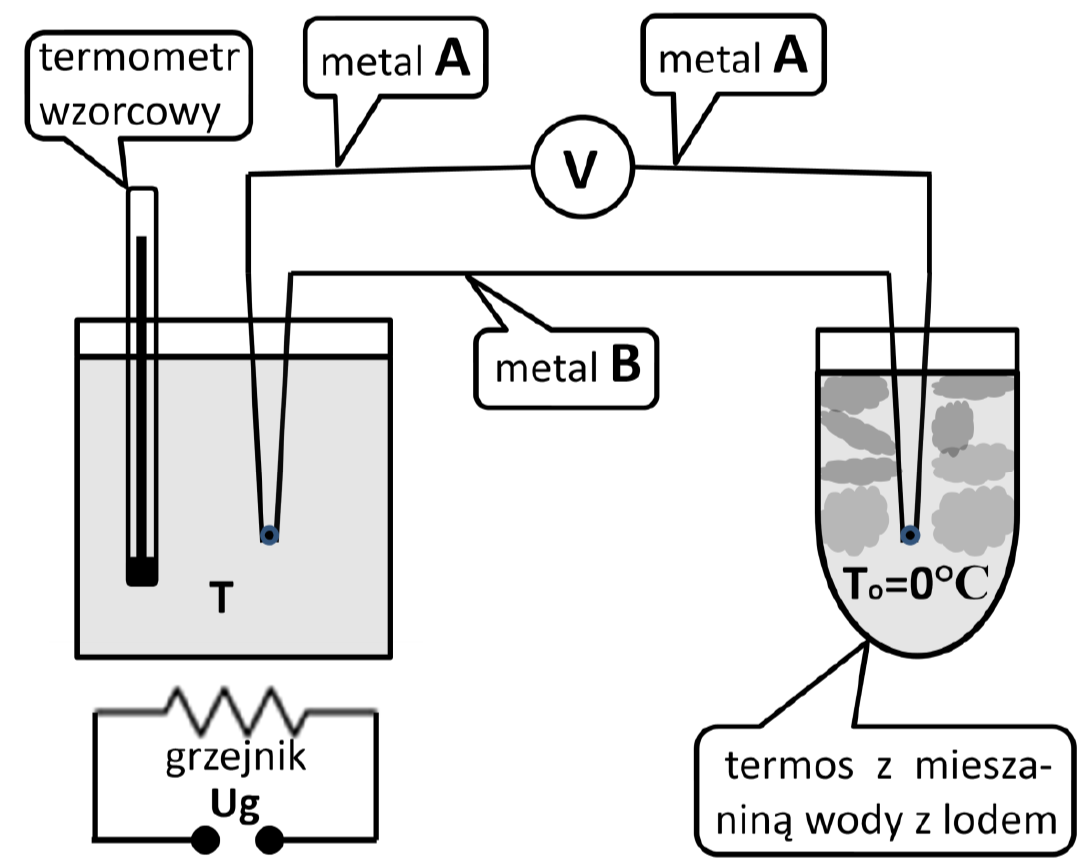
\includegraphics[width=8cm]{schemat_ukladu.png}
\end{figure}
Lepkość zostanie wyznaczona na podstawie danych otrzymanych przez obserwacje kulki 
tonącej w glicerynie. Dzięki analizie ruchu kulki, znając jej parametry takie 
jak masa i średnica, które przekładają się na gęstość. Można zanalizować siły oporu,
które stawia ciecz co przekłada się na współczynnik lepkości $\eta$.\\ \\
W naszym eksperymencie wykorzystamy następujące przyrządy:\\
\begin{itemize}
    \item Termomentr
    \item Garnek z wodą
    \item Termos wody z lodem
    \item Kuchenka
    \item Woltomierz
    \item Stoper
    \item Mieszadełko
    \item Tygiel ze stopem Wooda
    \item Podstawka chłodząca
\end{itemize}
% WSTEP TEORETYCZNY
\section{Skalowanie termopary i wyznaczenie współczynnika termoelektrycznego $\alpha$}
\begin{figure}[h]
    \begin{center}
    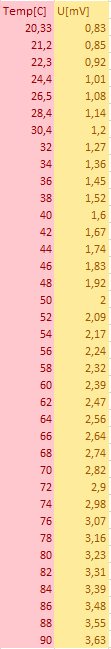
\includegraphics[scale=0.5]{wyniki.PNG}
    \end{center}
\end{figure}
Wzory:\\
niepewność multimetra\\
$u(U)=\frac{0,05}{100}\cdot U+0,001$\\

niepewność termometru\\
$u(T)=\pm0,01\degree$\\
\begin{figure}[h]
    \begin{center}
    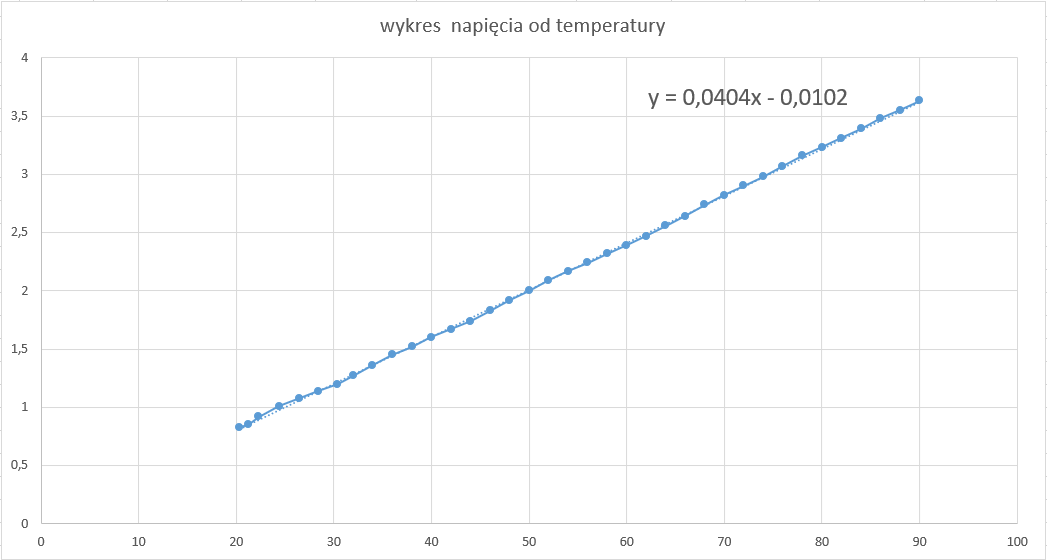
\includegraphics[width=14cm]{wykres.PNG}
    \end{center}
\end{figure}
Z regresji liniowej wynika, że $\alpha\approx0,0404\lbrack\frac{mV}{C}\rbrack$ natomiast jej błąd $u(\alpha)\approx0,00012$\\
\section{Wyznaczenie temperatury krzepnięcia stopu metali oraz niepewności jej
wyznaczenia}
\begin{figure}[h]
    \begin{center}
    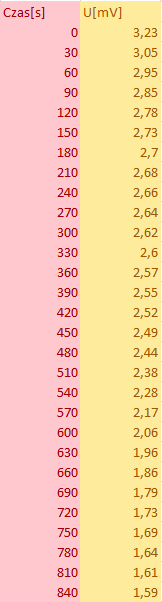
\includegraphics[scale=0.6]{wyniki2.PNG}
    \end{center}
\end{figure}
\begin{figure}[h]
    \begin{center}
    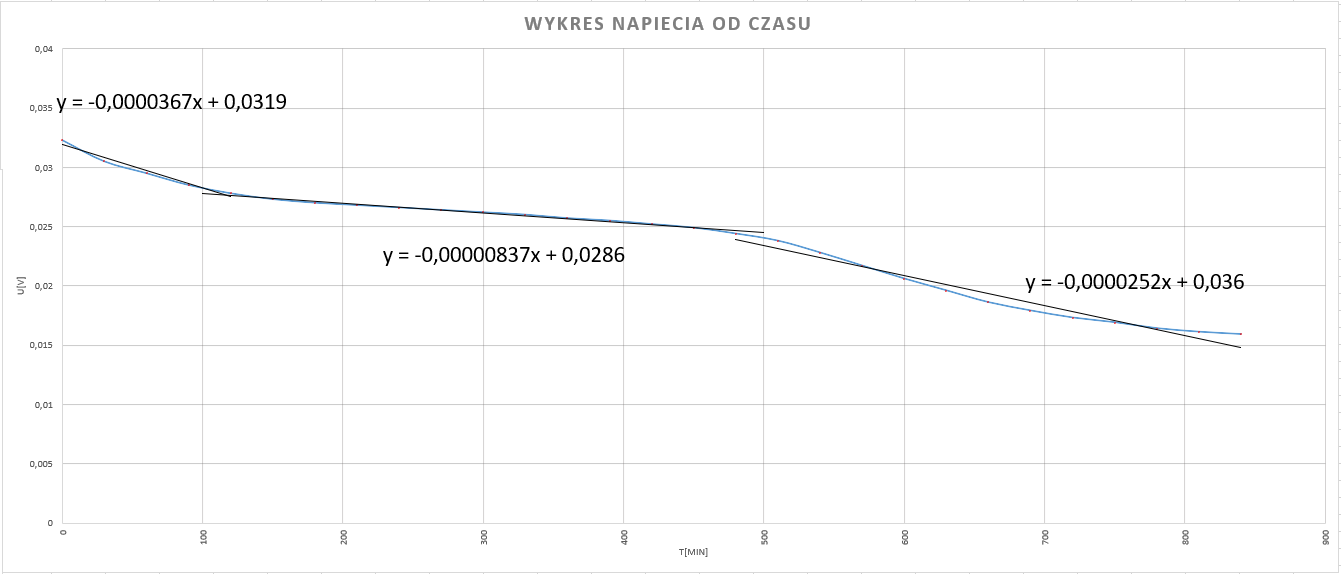
\includegraphics[width=16cm]{wykres2.PNG}
    \end{center}
\end{figure}
Wzory:\\
 niepewność standardowa typu A wartości
średniej napięć mieszczących się w obszarze plateau\\
$u_{A}(\overline{U})=\sqrt{\frac{\sum_{i=1}^{n}(U_{i}-\overline{U}_{i})^2}{n\cdot(n-1)}}$\\

niepewność standardowa typu B\\
$\Delta_{p}(U)=\frac{0,05}{100}\cdot U+0,001$\\

$u_{B}(U)=\frac{\Delta_{p}(U)}{\sqrt{3}}$\\

niepewność napięcia krzepnięcia można obliczyć ze wzoru\\
$u(U_{k})=\sqrt{(u_{A}(\overline{U}))^2+(u_{B}(U))^2}$\\

Przykładowe obliczenia:\\
$u_{A}(\overline{U})=\sqrt{\frac{\sum_{i=1}^{29}(U_{i}-\overline{U}_{i})^2}{29\cdot28}}\approx0,000022V$\\

$u_{B}(U)=\frac{\Delta_{p}(U)}{\sqrt{3}}\approx0,00059V$\\

$u(U_{k})=\sqrt{(0,0000216))^2+(0,000585)^2}\approx0,00059V$\\

Temperatura krzepnięcia stopu\\
$T_{k}=\frac{U_{k}}{\alpha}=\frac{2,62}{0,0404}\approx64,8C\degree$\\

$u_{c}(T_{k})\approx2,7C\degree$\\
\section{Wnioski}
\begin{itemize}
    \item wraz ze wzrostem temperatury przewodów rośnie napięcie
    \item podczas mierzenia przewodności stopu wooda w pewnym momencie spadek napięcia praktycznie znika, wynika to z powodu przejścia stanu skupienia stopu z ciekłego na stały
\end{itemize}
%trzeba dodać tabelki i te wykresy tak to wszystko powinno się zgadzać
%można jeszcze wnioski ale nie wiem jakie
%------------------------------------------------------------------
\end{document}
